	\section{The Mixed Side Principle} % (fold)
	\label{sub:the_mixedside_principle}
		The Mixed Side Principle is a fundamental constraint that the developer has to comply with when using MiCS. In a MiCS web application project there are three kinds of code the user can write; client side code (annotated with the \texttt{ClientSide} attribute), mixed side code (annotated with the \texttt{MixedSide attribute}) and server side code. The Mixed Side Principle describes a simple rule set for the interactions between the different kinds of code. 

		The Mixed Side Principle states that; \emph{Mixed side code can only use other mixed side code. Server and client side code can use mixed side code and code of their own kind.}

		The Mixed Side Principle is illustrated in Figure \ref{fig:MixedSidePrinciple}.

		\begin{figure}[H]
			\begin{center}
				\centerline{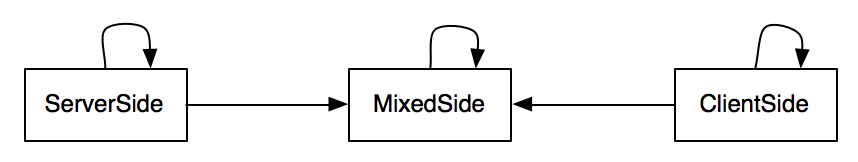
\includegraphics[width=12cm]{resources/images/MixedSidePrinciple.png}}
			\end{center}
			\caption{The Mixed Side Principle. Arrows indicate which kinds of code is can be used by a specific kind.}
			\label{fig:MixedSidePrinciple}
		\end{figure}

		Code annotated with the \texttt{ClientSide} attribute is only meant to be run on client side in form of generated JavaScript. Therefore client side code cannot make calls to server side only objects. This would not make sense as server and client side are two different and separated execution contexts.  If client side code were to call server side code, it would ultimately result in a client side error as the server side code will not be mapped to client side JavaScript. Likewise it will not make sense for server side code to call client side code.

		Code annotated with the \texttt{MixedSide} attribute can be called both from client and server side code. Mixed side code can only call other mixed side code and therefore it cannot use client side only types, such as DOM types. This would simply not make sense when mixed side code is called from server side.

		All three kinds of code can obviously use other code of the same kind hence the recursive arrows in illustartion \ref{fig:MixedSidePrinciple}.